
\begin{frame}
  \frametitle{UMI-Count vs TPM}
  \begin{itemize}
  \item
    Data set: PBMC scRNAseq data \cite{yuen2020high}, 10 individuals, 5 vs 5 in
    two conditions.
  \item
    Select genes:
    \begin{itemize}
    \item
      DEGs: CCL4L1, CCL4L2, CCL3L1, CCL3L3
    \item
      Genes with lots of zeros: MIR155HG, TNFRSF4, ICAM1, NA.499, HIST2H2AA4
    \item
      Genes with strong individual effects: HBB, HBA2, HBA1 
    \end{itemize}
  % \item
    % \(\log_2CPM\) for the gene \(i\) in the cell is defined as \(log_2(\frac{X_g}{\sum_g X_g} \times C + 1)\), C is a
    % constant, defined as \(10^4\) in Seurat.
  \end{itemize}
\end{frame}

\begin{frame}
  \frametitle{What is a violin plot?}
  Violin plots are similar to box plots, except that they also show the kernel
  probability density of the data at different values.
  \begin{figure}
    \centering
    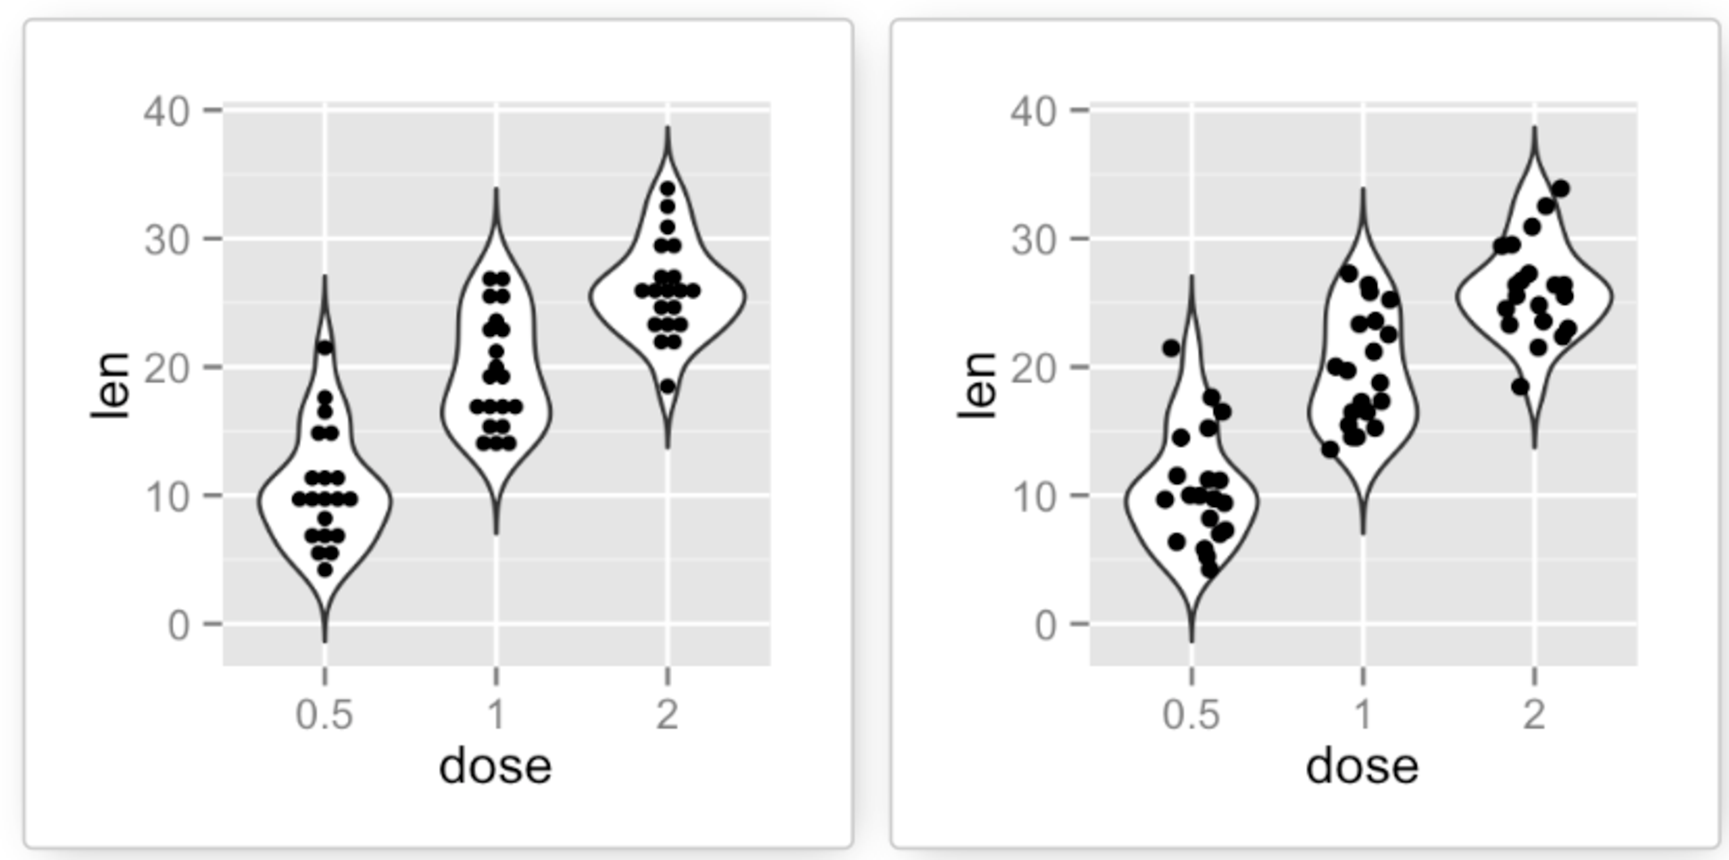
\includegraphics[width = 0.8\textwidth]{violin_figure_case}
    \caption{Violin plot. Left: Dotplot, where each dot corresponds to one
      sample; Right: Jitter plot, which adds small randomness to the data in
      order to reduce the overlap among the points.}
  \end{figure}
\end{frame}

\begin{frame}
  \frametitle{DEGs in all cells}
  \begin{figure}
    \centering
    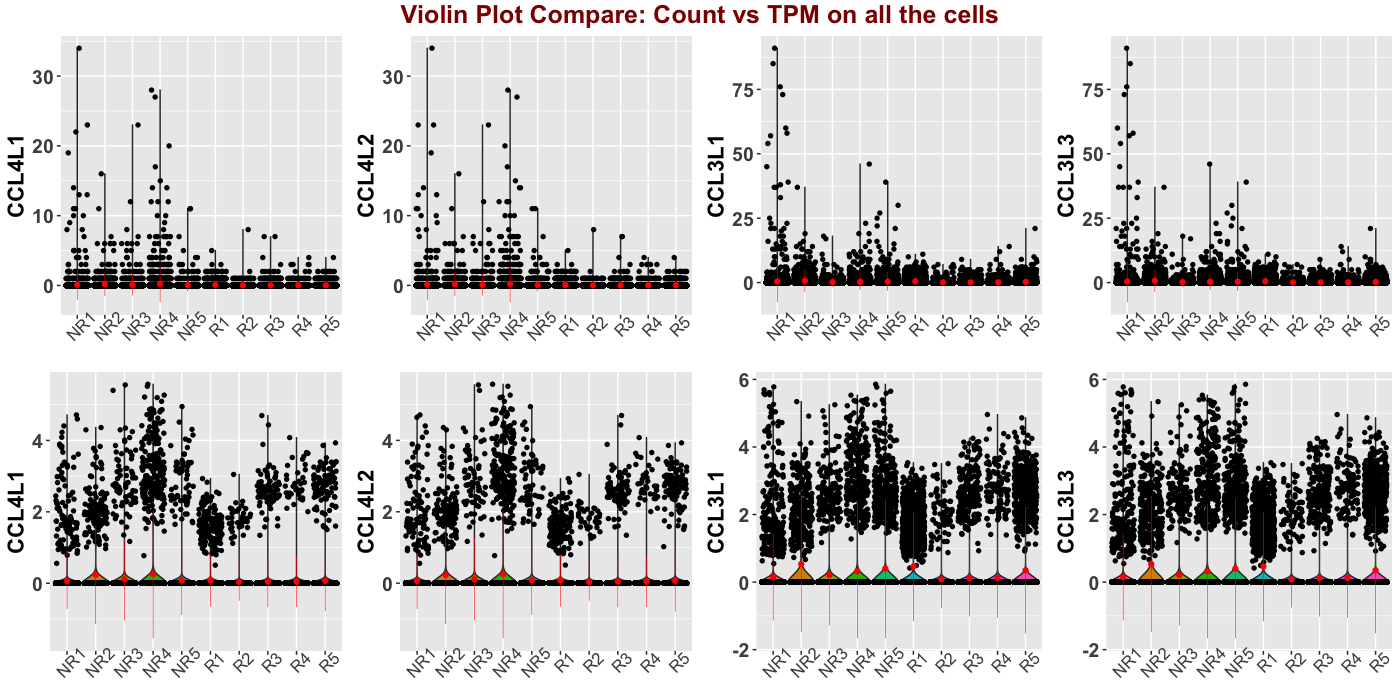
\includegraphics[width=\textwidth]{vln_cnt-tpm_DEGs_allcells}
  \end{figure}
\end{frame}

\begin{frame}
  \frametitle{DEGs in cytotoxic T cells}
  \begin{figure}
    \centering
    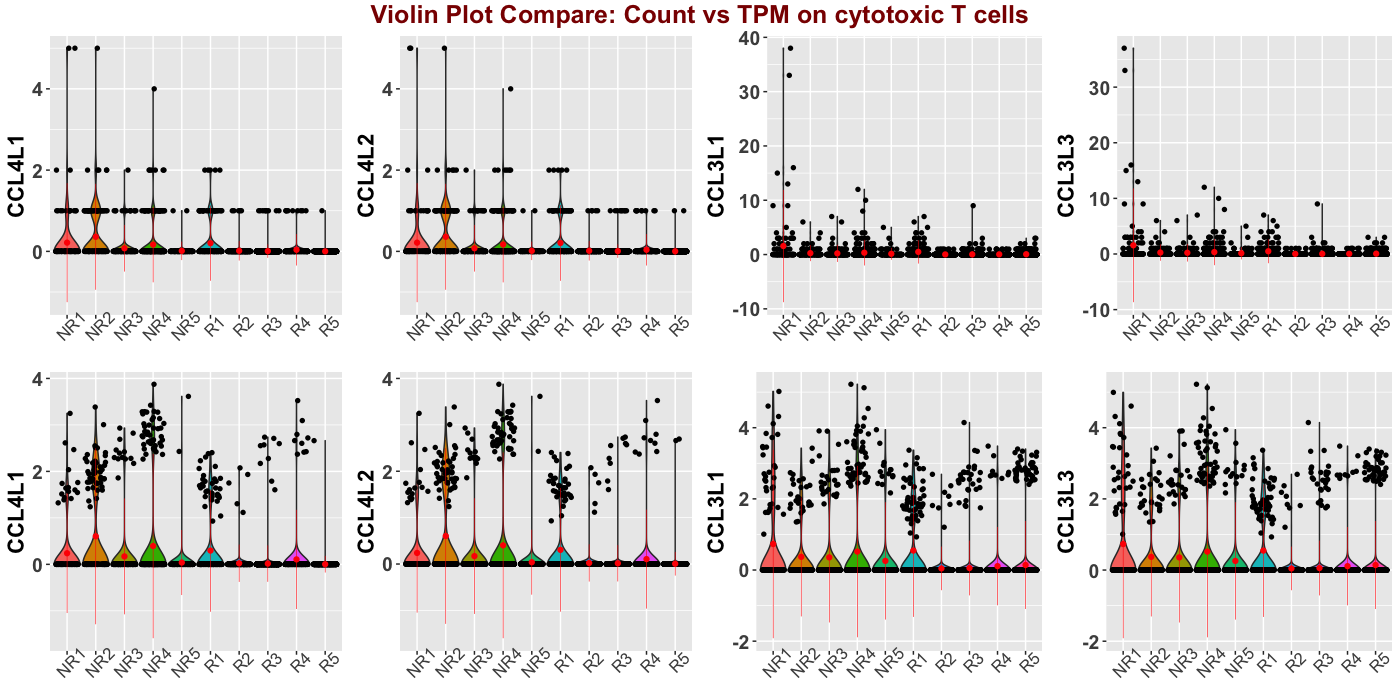
\includegraphics[width=\textwidth]{vln_cnt-tpm_DEGs_cytotoxicTcell}
  \end{figure}
\end{frame}

\begin{frame}
\frametitle{Genes with lots of zeros in all cells}
\begin{figure}
  \centering
  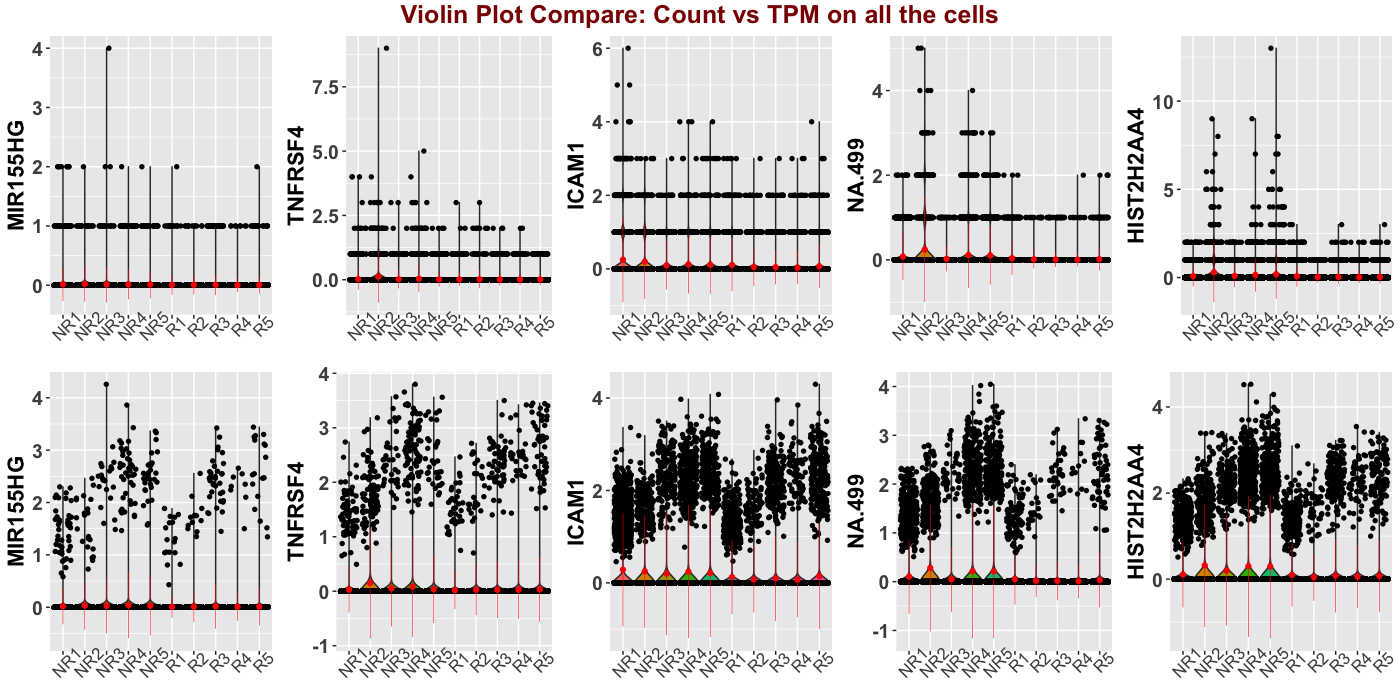
\includegraphics[width=\textwidth]{vln_cnt-tpm_heavyzeros_allcells}
\end{figure}
\end{frame}

\begin{frame}
  \frametitle{Genes with lots of zeros in cytotoxic T cells}
  \begin{figure}
    \centering
    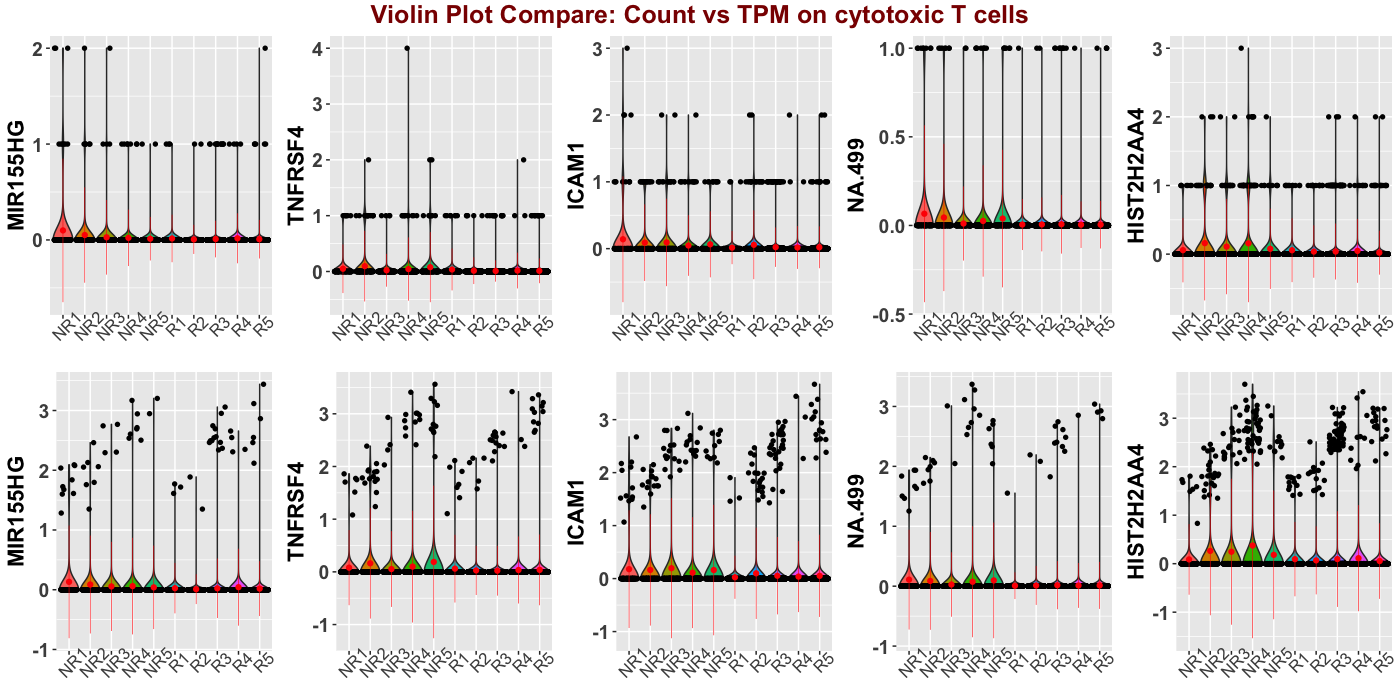
\includegraphics[width=\textwidth]{vln_cnt-tpm_heavyzeros_cytotoxicTcell}
  \end{figure}
\end{frame}

\begin{frame}
\frametitle{Genes with strong individual effects in all cells}
\begin{figure}
  \centering
  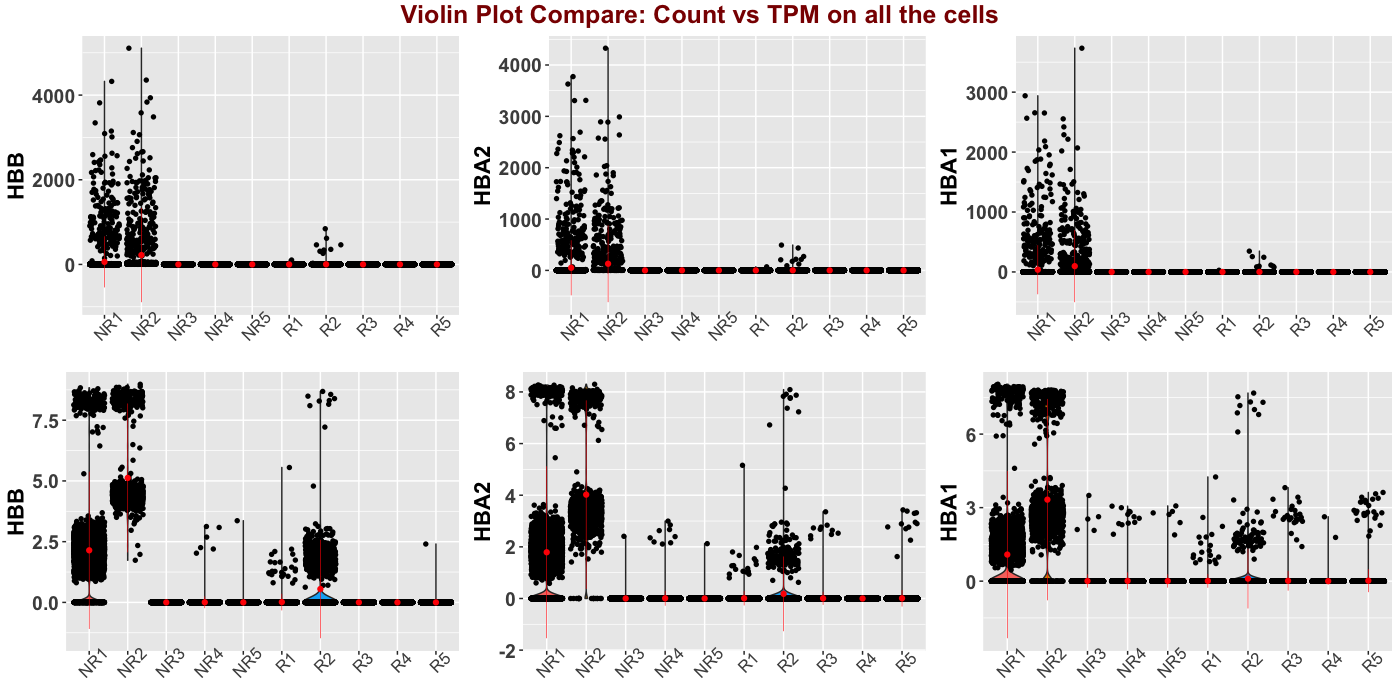
\includegraphics[width=\textwidth]{vln_cnt-tpm_heavyindeff_allcells}
\end{figure}
\end{frame}

\begin{frame}
  \frametitle{Genes with strong individual effects in cytotoxic T cells}
  \begin{figure}
    \centering
    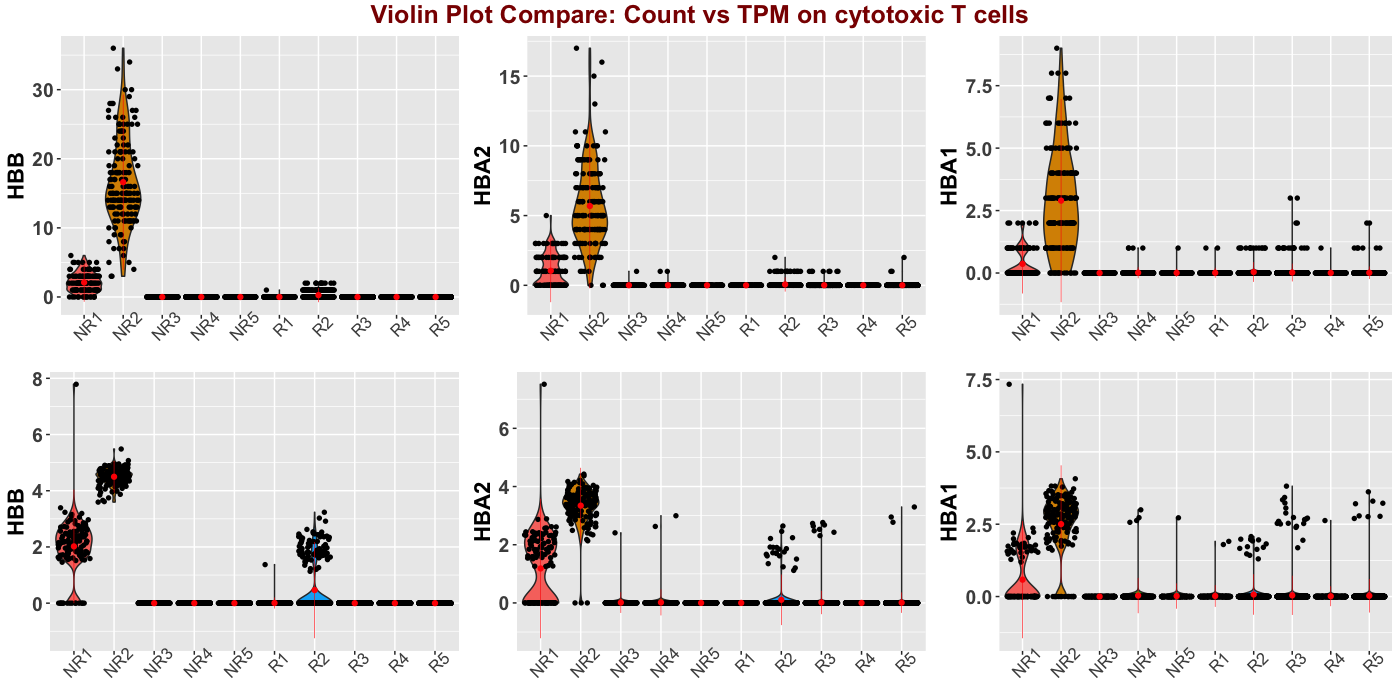
\includegraphics[width=\textwidth]{vln_cnt-tpm_heavyindeff_cytotoxicTcell}
  \end{figure}
\end{frame}

\begin{frame}
  \frametitle{Multinomial model on scRNASeq \cite{townes2019feature}}
  Under a multinomial distribution on the observed UMI counts, 74\%-90\%
  zeros, 22-30\% ones, and less than 4\% values above one. This will
  artificially enhance the gap between zero and nonzeros values on
  log-normalized data.
  \begin{figure}
    \centering
    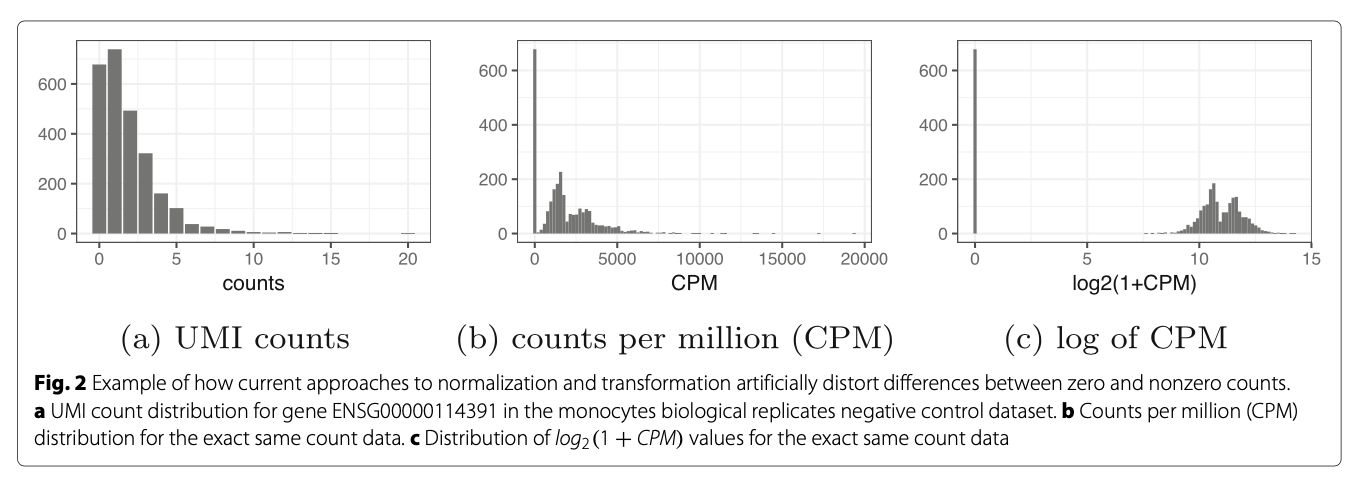
\includegraphics[width=\textwidth]{lognorm_artificial_zeroinflation}
  \end{figure}
\end{frame}

